\chapter{Implementation}
\label{chap:implem}
\section {Development environment overview}
Incremental recogniser is implemented in Java programming language, using
an open-source project \textit {Incremental Spoken Dialogue processing
Toolkit}(InproTK), developed by the Universities of Potsdam, Bielefeld and
Hamburg. InproTK includes modules for speech recognition, speech understanding,
speech processing and dialogue management.
Speech recognition module is based on implemented Java Sphinx-4 recogniser, a
package of CMUSphinx speech recognition toolkit. 
\section {IU Modules and Data Processing}
\textit {Incremental Units} (IU) are minimal data processing unit in InptoTK.
They are interconnected with each, forming a network of IUs \parencite
{baumann2013:phd}.

\begin{figure}[htbp]
  \centering
    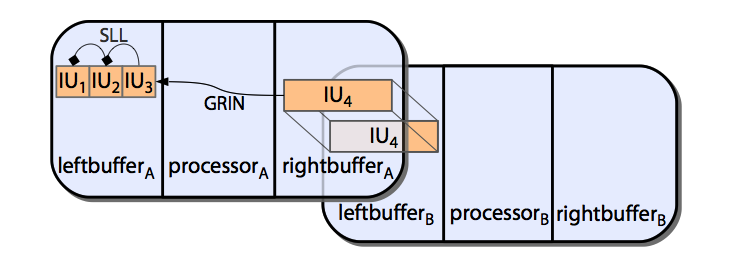
\includegraphics[width=1.0\textwidth]{images/iuandbuffer.png}
 \caption{ Incremental Units (IUs) and their intercommunication via left-right
 buffers \parencite {baumann2013:phd}}
  \label{fig:Bild1}
\end {figure}
\subsection {GoogleASR Module in InproTK}
GoogleASR is a source IU in InproTK, which listens to results coming from
Google's  downstream connection in JavaScript Object Notation (JSON) format and
passes results to its listeners by updating the current hypotheses and providing
info about the hypotheses time (hypotheses start and end times).
 \begin{figure}[htbp]
  \centering
   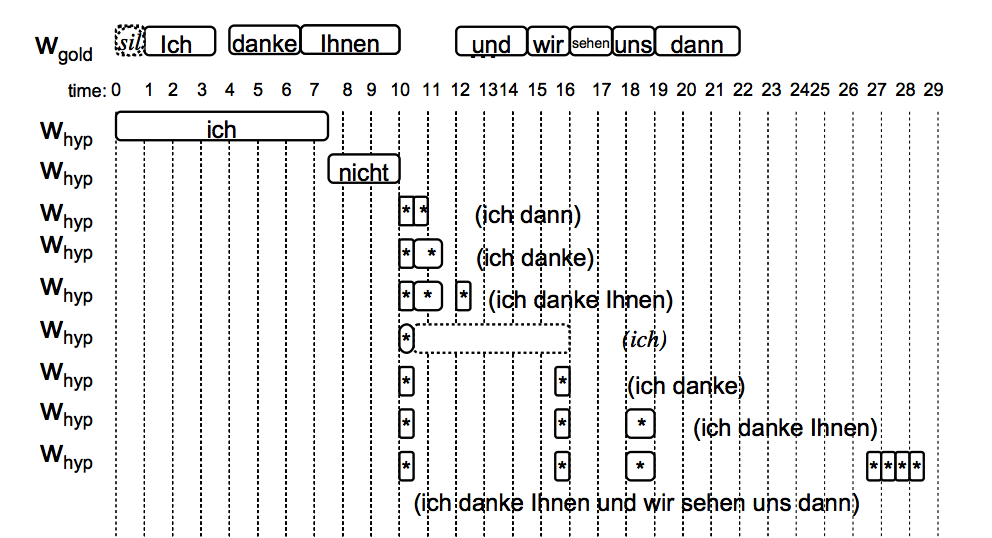
\includegraphics[width=0.9\textwidth]{images/google_output.png}
  \caption{Incremental output of Google ASR with existing timing}
  \label{fig:google_ouput}
\end{figure}

Timing, implemented in Google ASR, has nothing to do with true alignment.
With the help of this information  it is only possible to calculate the
timeliness: FO as well as FD.  Manual reconstruction of alignment from
timeliness is problematic as timeliness does not preserve any information about word
duration. 


For example, in the picture  \ref {fig:google_ouput} the first hypotheses (word ``ich) equals 0
and end times equals about 7.5 time slots, whereas the borders of the word
``ich'' are between 1 and 3.5 time slot. In addition, in case of Google we are dealing with additional output delay,
resulted from network latency, which can be slightly variable approximately
between 50 and 200 ms. Google has processed the file till the end of the word
``ich'' by the time 3.5, after some internal Google offset, the output was made.
It is assumed, that Google offset reflects the problem of stability of the
the output and latency \parencite {mcgrawgrauenstein2012}. Finally, Google ASR returned this result after 
network delay.  
 \begin{figure}[htbp]
  \centering
   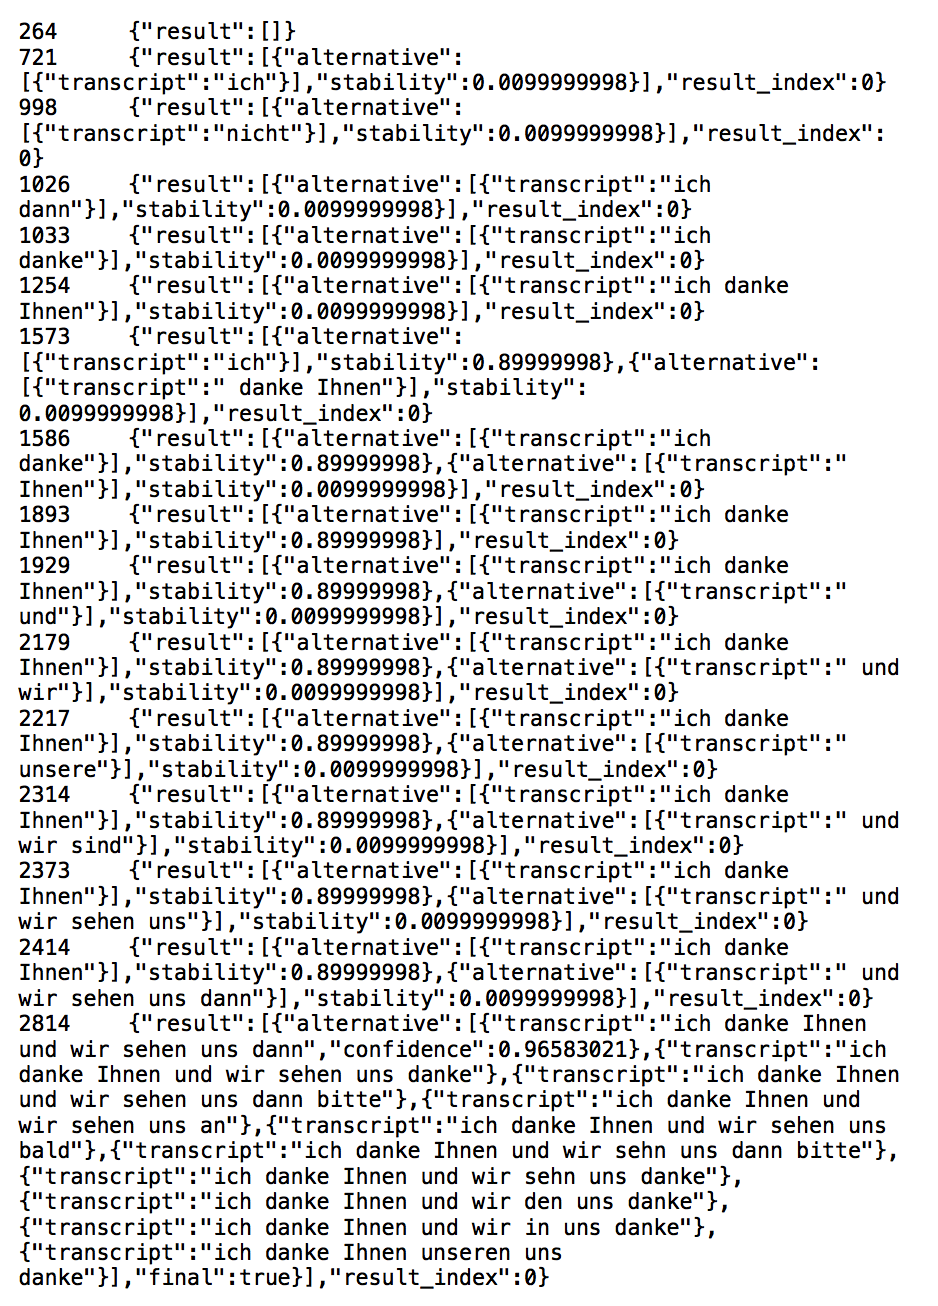
\includegraphics[width=1\textwidth]{images/json.png}
    \caption{JSON file example}
      \label{fig:json_ouput}
\end{figure}
\subsection {SphinxASR Module}
\section {Architecture of the Implemented combined Google-Sphinx Recognizer}
Sphinx-Google architecture includes Sphinx-4 frontend, dictionary,
language model and acoustic model, decoder with search graph, forced-alignment
module, Sphinx control thread, synchronous blocking queue and InproTK IUs:
Google ASR, Sphinx ASR and label writer.  (see figure \ref {fig:arch}).
\begin{figure}[htbp]
  \centering
    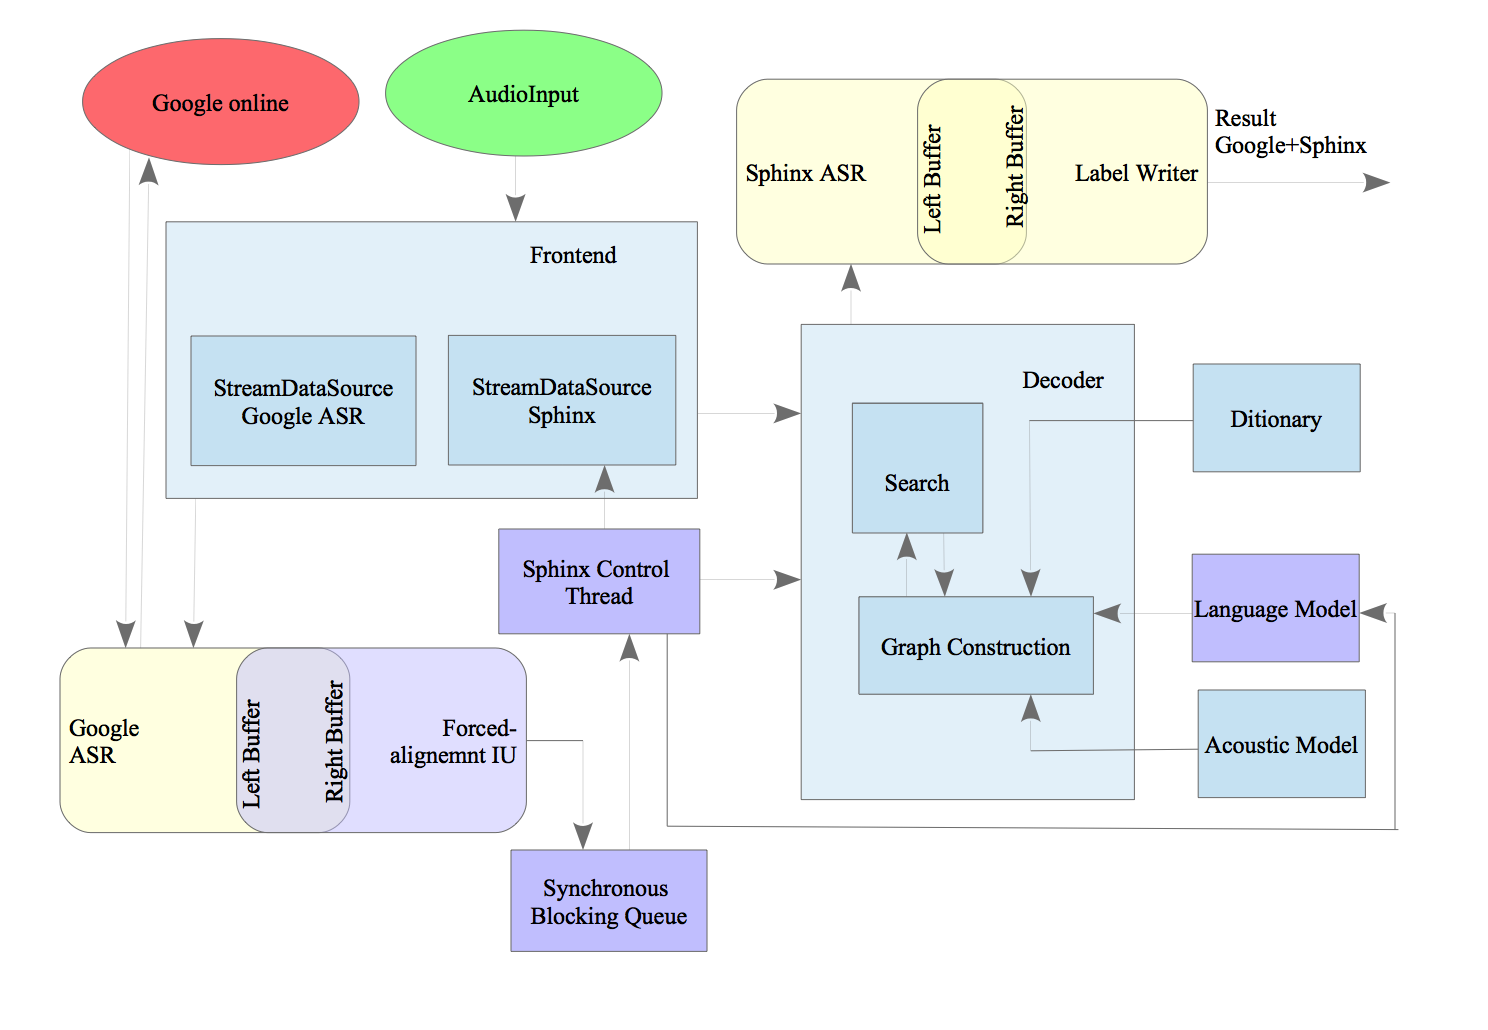
\includegraphics[width=1\textwidth]{images/architecture.png}
 \caption{Implementation Overview}
  \label{fig:arch}
\end {figure} 
%\subsection {Frontend}

As an audio input both Google ASR and Sphinx receive the same audio input.
Input stream of Google ASR is set only once, whereas the length of
the stream is equal to the whole audio. By contrast, the Sphinx input stream is
updated every time, Google ASR returns new hypothesis. 

GoogleASR listens to JSON results coming from online Google, running
in incremental mode, and passes result to forced-alignment IU. Google ASR result
is transferred to forced-alignment IU via standard IU left-right buffer. Google
ASR result contains hypothesis, and the start and end times, computed by Google
ASR for every hypothesis. 

Forced-alignment IU puts every incremental Google result into synchronous
blocking queue. Sphinx control thread takes the last Google hypothesis from the
synchronous blocking queue and starts Sphinx decoding. Sphinx control thread
updates language model, resetting text for alignment. As soon as the grammar of
the language model is changed, search graph of the decoder module is rebuild
anew. 

Every time the new hypothesis is taken from the queue Sphinx input stream  is
also reset. The length of this stream is a part of the audio input.  


Sphinx returns not only alignment result, based on Google ASR, but continues
with recognition, while waiting for the new Google incremental result. 

The initialisation and implementation of the SearchGraph is realised by
Sphinx-4. The choice and alternation of the path in
the SearchGraph depends on the Google incremental hypotheses. 
When the new Google hypotheses differs from the present hypotheses in the
SearchGraph, the SearchGraph is reseted and the hypotheses path is
corrected.  Timeliness improvement is supposed to be achieved by faster results
produced by Sphinx, whereas the path in the Sphinx SearchGraph is predetermined
by Google incremental result. The last means that we get the same final results
for Google and Google + Sphinx, but timeliness of Google + Sphinx
is expected to be improved. 



\section {Forced-alignment of Google Incremental Results with Google-Sphinx
Recognizer}
\section {Search Module of Google-Sphinx Recognizer}
\subsection {Decoder configuration}
\subsection {Search Modification}